\chapter{Introduction}\label{chap:intro}

\section{Background}\label{sect:background}

Depth estimation from stereo image pairs is about inferring the depth
of each pixel, essentially adding a third dimension to a 2-dimensional
image. Many applications can benefit from this information; one of the
earliest uses was in the field of photogrammetry for automatically
constructing topographic elevation maps from aerial images. In
robotics, depth information is vital for navigation and manipulation.
3D reconstruction from images can enable view interpolation and
image-based rendering, allowing a user to freely chose a synthetic
view-point other than the views straight out of the cameras.

Figure \ref{fig:applications-of-depth-information}, borrowed from
Richard Szeliskis excellent book \textit{Computer Vision: Algorithms
  and Applications}\cite{computer-vision-book} shows some of the more
recent uses researchers have been able to create with depth
information.

\begin{figure}
  \label{fig:applications-of-depth-information}
  \centering

  \begin{subfigure}[b]{0.3\textwidth}
    \centering
    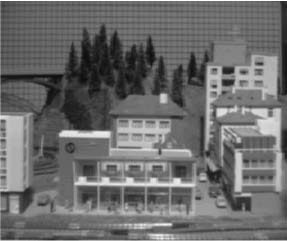
\includegraphics[width=\textwidth]{images/input.png}
    \caption{}
  \end{subfigure}
  ~
  \begin{subfigure}[b]{0.3\textwidth}
    \centering
    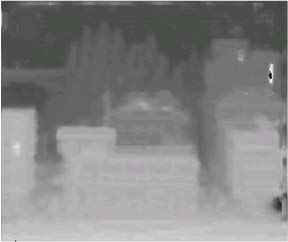
\includegraphics[width=\textwidth]{images/computed-depth.png}
    \caption{}
  \end{subfigure}
  ~
  \begin{subfigure}[b]{0.3\textwidth}
    \centering
    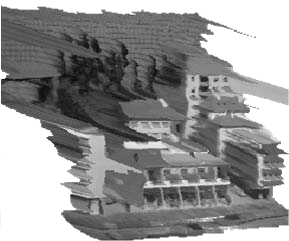
\includegraphics[width=\textwidth]{images/synthesized-view.png}
    \caption{}
  \end{subfigure}

  % newline

  \begin{subfigure}[b]{0.24\textwidth}
    \centering
    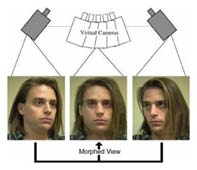
\includegraphics[width=\textwidth]{images/three-view.png}
    \caption{}
  \end{subfigure}
  ~
  \begin{subfigure}[b]{0.2\textwidth}
    \centering
    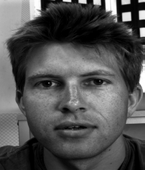
\includegraphics[width=\textwidth]{images/input-face.png}
    \caption{}
  \end{subfigure}
  ~
  \begin{subfigure}[b]{0.2\textwidth}
    \centering
    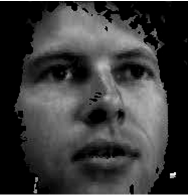
\includegraphics[width=\textwidth]{images/synthesized-face.png}
    \caption{}
  \end{subfigure}
  ~
  \begin{subfigure}[b]{0.2\textwidth}
    \centering
    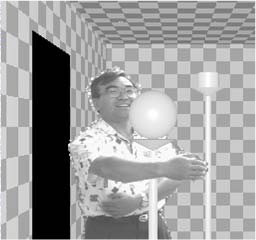
\includegraphics[width=\textwidth]{images/z-key.png}
    \caption{}
  \end{subfigure}

  % newline

  \begin{subfigure}[b]{0.3\textwidth}
    \centering
    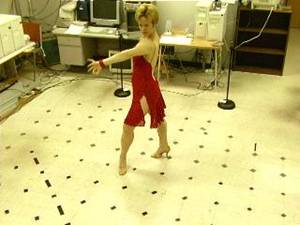
\includegraphics[width=\textwidth]{images/3d-input-left.png}
    \caption{}
  \end{subfigure}
  ~
  \begin{subfigure}[b]{0.3\textwidth}
    \centering
    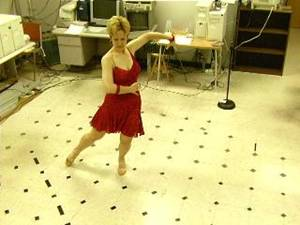
\includegraphics[width=\textwidth]{images/3d-input-right.png}
    \caption{}
  \end{subfigure}
  ~
  \begin{subfigure}[b]{0.3\textwidth}
    \centering
    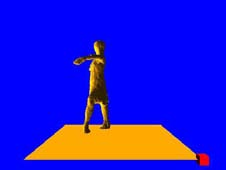
\includegraphics[width=\textwidth]{images/3d-reconstruction.png}
    \caption{}
  \end{subfigure}

  \caption{Applications of stereo vision: (a) input image, (b)
    computed depth map, and (c) new view generagtion from multi-view
    stereo \cite{matthies-kanade-szeliski}; (d) view morphing between
    two images \cite{seitz-dyer}; (e-f) 3D face modeling (images
    courtesy of Frederic Devernay); (g) z-keying live and
    computer-generated imagery \cite{kanade-yoshida-oda}; (h-j)
    building 3D surface models from multiple video streams in
    Virtualized Reality \cite{kanade-rander-narayanan}}
\end{figure}

\section{Problem Statement}\label{sect:prob-statement}

There are plenty of algorithms for disparity calculations. They all
have their characteristics; fast but coarse quality, good quality but
slow, good at object boundary but bad at continuous textureless areas.
These have all been researched heavily for decades, but has until
recently been very limited by the processing power of the days
computers. With the advent of cheap parallel computing devices in the
form of cheap consumer GPUs and cheap multi-cored CPUs, and frameworks
such as OpenCL and CUDA maturing, super-computer-like number crunching
has never been so fast and easy to do on home computers.

The goal of this thesis is to provide an implementation of the
algorithm most likely able to achieve real time estimation with High
Definition input.


\section{Main Contributions}\label{sect:contributions}

The main contribution of this thesis is a working OpenCL
implementation for GPUs able to run the depth estimation pipeline in
real time on high definition images. The evolution from a simple CPU
implementation to the final real time GPU implementation is documented
and analyzed, including many of the GPU architecture optimizations
approaches.

The secondary contribution is the \textit{compute mask} technique.
Sequential video frames contain a lot of redundant information. This
is especially true for statically mounted cameras filming some scene,
i.eg a theater stage. In such a scenario, the only moving objects in
the frames will often be just an actor or two, making the calculation
of the background redundant since it will result in the same value as
in the previous frame. The compute mask is a binary map indicating
whether a pixel needs to be calculated, or if the disparity value can
be copied from the disparity map of the previous frame.

\section{Limitations}\label{sect:limitations}

\subsubsection{Discretized disparity space}

The implementation produces 8-bit single channel gray-scale disparity
maps of the same dimensions as the input, which limits the number of
disparity levels to 256. This level of quantization may be fine for
some applications, like robotic navigation, but can lead to
unappealing results for other applications, like image-based view
synthesis.

\subsubsection{Camera calibration and Stereo rectification}
Input images must be stereo rectified. For a block matching algorithm
to be as effective as possible, it has to be able to assume that
corresponding points lie along the horizontal scan-line
(x-axis). Stereo rectification and camera calibration is such a
well-understood topic in computer vision, that most stereo
correspondence algorithms assumes its cameras are calibrated and the
inputs are rectified. 

\begin{figure}

  \begin{subfigure}[b]{0.48\textwidth}
    \centering
    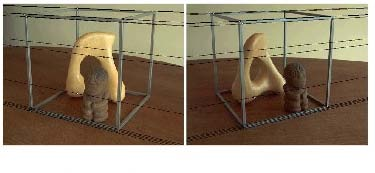
\includegraphics[width=\textwidth]{images/rectification-example.png}
    \caption{}
  \end{subfigure}
  ~
  \begin{subfigure}[b]{0.48\textwidth}
    \centering
    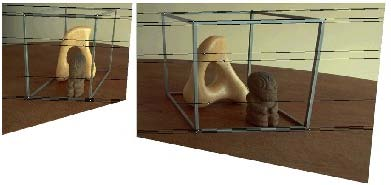
\includegraphics[width=\textwidth]{images/rectification-example-2.png}
    \caption{}
  \end{subfigure}

  \begin{subfigure}[b]{0.48\textwidth}
    \centering
    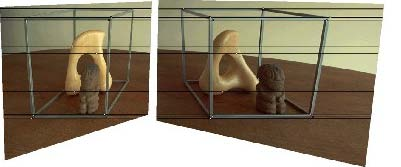
\includegraphics[width=\textwidth]{images/rectification-example-3.png}
    \caption{}
  \end{subfigure}
  ~
  \begin{subfigure}[b]{0.48\textwidth}
    \centering
    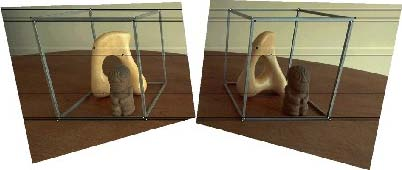
\includegraphics[width=\textwidth]{images/rectification-example-4.png}
    \caption{}
  \end{subfigure}

  \caption{An example showing various stages of Loop and
    Zhangs\cite{loop-zhang} proposed rectification algorithm. (a)
    Original image pair overlaid with several epipolar lines; (b)
    Image pair transformed so that epipolar lines are parallel to each
    other in each image; (c) Rectified image pair; (d) Final shearing
    transformation}

\end{figure}

To convert the disparity values to depth values, the intrinsic and
extrinsic matrices from the cameras that took the input images must be
provided. More specifically, the baseline (distance between the two
cameras) and the lenses focal length is needed in a formula, as will
be explained in chapter \ref{sec:depthestimation_theory}.

\section{Outline}

Chapter \ref{sect:design} presents the core ideas of stereo depth
estimation in computer vision, and related work.

The OpenCL framework is presented in chapter \ref{sect:arch} along with
some optimization strategies for GPU devices.

In chapter \ref{sect:impl}, the implementation is presented. It starts
off with the most basic depth estimator CPU implementation, followed
by an as direct as possible port to OpenCL. From there, various
optimizations are applied, followed finally by the refinement kernels.

The last chapter, \ref{sect:eval}, evaluates the results
